\documentclass[12pt]{article}
\usepackage[left=0.25cm,top=1cm,right=0.25cm,bottom=1cm]{geometry}
\textwidth = 20cm
\hoffset = -1cm
\usepackage[utf8]{inputenc}
\usepackage[spanish,es-tabla]{babel}
\usepackage[autostyle,spanish=mexican]{csquotes}
\usepackage[tbtags]{amsmath}
\usepackage{nccmath}
\usepackage{amsthm}
\usepackage{amssymb}
\usepackage{graphicx}
\usepackage{standalone}
\usepackage[outdir=./]{epstopdf}
\usepackage{siunitx}
\usepackage{physics}
\usepackage{color}
\usepackage{float}
\usepackage{multicol}
%\usepackage{milista}
\usepackage{enumitem}
\usepackage{anyfontsize}
\usepackage{anysize}
\usepackage{enumitem}
\usepackage{capt-of}
\usepackage{bm}
\usepackage{relsize}
\usepackage{placeins}
\usepackage{empheq}
\usepackage{cancel}
\usepackage{wrapfig}
\spanishdecimal{.}
\renewcommand{\baselinestretch}{1.5} 
\renewcommand\labelenumii{\theenumi.{\arabic{enumii}}}
\newcommand{\ptilde}[1]{\ensuremath{{#1}^{\prime}}}
\newcommand{\stilde}[1]{\ensuremath{{#1}^{\prime \prime}}}
\newcommand{\ttilde}[1]{\ensuremath{{#1}^{\prime \prime \prime}}}
\newcommand{\ntilde}[2]{\ensuremath{{#1}^{(#2)}}}


\title{Ecuación de Laplace en esferas} \vspace{-3ex}
\author{M. en C. Gustavo Contreras Mayén}
\date{ }
\newcommand{\Cancel}[2][black]{{\color{#1}\cancel{\color{black}#2}}}
\begin{document}
\vspace{-4cm}
\maketitle
\fontsize{14}{14}\selectfont
\tableofcontents
\newpage

\section{Problema a resolver.}
\subsection{Semiesferas a distintas temperaturas}

Considera el siguiente problema: Dos hemisferios sólidos conductores de calor de radio $a$, separados por un pequeño espacio aislante, forman una esfera. Las dos mitades de la esfera están en contacto, en el exterior, con dos baños de calor (infinitos) a temperaturas $T_{0}$ y $-T_{0} $, ver la figura (\ref{fig:figura_esfera_01}):
\begin{figure}[H]
    \centering
    \includegraphics[scale=1.3]{Imagenes/Ejemplo_Esfera_01.eps}
    \caption{Dos hemisferios a distintas temperaturas.}
    \label{fig:figura_esfera_01}
\end{figure}

\textbf{Queremos encontrar la distribución de temperatura $T(r, \theta, \varphi)$ en puntos dentro de la esfera.}

\section{Ecuación de Laplace.}
\subsection{Coordenadas esféricas.}

Dada la simetría esférica del problema, es directa la relación de trabajo con un sistema coordenado esférico $(r, \theta, \varphi)$.
\par
Tomando la ecuación de Laplace como punto de partida, habrá que expresarla en las coordenadas esféricas. Como ya sabemos hacer el cambio entre el sistema cartesiano y el esférico, la ecuación de Laplace se expresa como:
\begin{align}
\dfrac{1}{r^{2}} \pdv{r} \left( r^{2} \pdv{\Psi}{r} \right) + \dfrac{1}{r^{2} \, \sin \theta} \bigg[ \pdv{\theta} \left( \sin \theta \pdv{\Psi}{\theta} \right) + \dfrac{1}{\sin \theta} \, \pdv[2]{\Psi}{\varphi} \bigg] = 0
\label{eq:ecuacion_22_15}
\end{align}

\subsection{Separación de variables.}

Para ocupar la técnica de separación de variables, proponemos una solución del tipo:
\begin{align*}
\Psi(r, \theta, \varphi) = R(r) \Theta (\theta) \Phi(\varphi)
\end{align*}
Que sustituimos en la ec (\ref{eq:ecuacion_22_15}).
\par
En el necesario paso de separar la ecuación en expresiones que dependan de una sola variable, en nuestro caso abreviamos el desarrollo. Pero en el camino encontramos \emph{dos constantes de separación}: $\alpha$ y $\beta$.
\par
Tendremos tres ecuaciones diferenciales ordinarias, mucho más fácil de resolver que la ecuación diferencial parcial:
\begin{enumerate}
\item Ecuación radial: La ED02OH que depende solo de la variable $r$ es:
\begin{align}
\dfrac{1}{r^{2}} \dv{r} \left( r^{2} \dv{R}{r} \right) - \dfrac{\alpha}{r^{2}} R = 0
\label{eq:ecuacion_26_1a}
\end{align}
a esta ecuación se le llama: la \textbf{ecuación radial}.
\item Ecuación polar: La ecuación que depende solo de $\theta$ es:
\begin{align}
\dfrac{1}{\sin \theta} \dv{\theta} \left( \sin \theta \dv{\Theta}{\theta} \right) + \left( \alpha - \dfrac{\beta}{\sin^{2} \theta} \right) \Theta = 0
\label{eq:ecuacion_26_1b}
\end{align}
esta es la \textbf{ecuación polar}.
\item Ecuación azimutal: La ecuación que depende del ángulo azimutal $\varphi$, es:
\begin{align}
\dv[2]{\Phi}{\varphi} + \beta \Phi = 0
\label{eq:ecuacion_26_1c}
\end{align}
es la llamada \textbf{ecuación azimutal.}
\end{enumerate}

Con la ecuación azimutal haremos una importante consideración: En casos donde sea conocido de antemano que el potencial sea independiente del ángulo azimutal $\varphi$, entonces el problema presenta una \textbf{simetría azimutal}.
\par
En este caso, podemos suponer que se tiene una función constante $S$, tal que:
\begin{align*}
\dv[2]{S}{\varphi} + \beta S = 0
\end{align*}
Esto implica que $\beta = 0$, ya que $S$ es una función contante no nula.
\par
Dejando para el problema de la ecuación de Laplace en coordenadas esféricas, un sistema de EDO2H reducido a dos expresiones:
\begin{align}
\begin{aligned}
\dfrac{1}{r^{2}} \dv{r} \left( r^{2} \dv{R}{r} \right) - \dfrac{\alpha}{r^{2}} R &= 0 \\[1em]
\dfrac{1}{\sin \theta} \dv{\theta} \left( \sin \theta \dv{\Theta}{\theta} \right) + \alpha \Theta &= 0
\end{aligned}
\label{eq:ecuacion_26_02}
\end{align}

\section{Resolviendo las EDO2H.}

\subsection{Ecuación polar.}

De manera inicial nos enfocamos en la ecuación polar. La presencia en el denominador del término $\sin \theta \dd{\theta}$ (que es el diferencial de $\cos \theta)$ sugiere el cambio de variable de $\theta$ a $u \equiv \cos \theta$.
\par
Para cualquier función $f(\theta)$, con la regla de la cadena se tiene:
\begin{align*}
\dv{f}{u} =  \dv{f}{\theta} \dv{\theta}{u} =  \dv{f}{\theta} \dfrac{1}{\dv*{u}{\theta}} =  - \dfrac{1}{\sin \theta} \dv{f}{\theta}
\end{align*}
De manera equivalente:
\begin{align}
\dv{f}{\theta} = - \sin \theta \dv{f}{u}
\label{eq:ecuacion_26_03}
\end{align}

Esto nos permite convertir la derivada de una función con respecto a $u$, en la derivada de la misma función con respecto a $\theta$.
\par
Proponemos una función $P(u)$ tal que:
\begin{align*}
P(u) = \Theta(\theta)
\end{align*}

Usamos la regla de la cadena mostrada, sustituyendo en la ecuación polar y escribiendo $\sin^{2} \theta = 1 - u^{2}$, la EDO pasa a ser:
\begin{align*}
- \dfrac{1}{\sin \theta} \dv{\theta} \bigg[ (1 - u^{2}) \dv{P}{u} \bigg] + \alpha P = 0
\end{align*}
El término en el corchete es función de $u$.
\par
Ocupando la ec. (\ref{eq:ecuacion_26_03}), podemos convertir la derivada en $\theta$ en una derivada en $u$, para así obtener:
\begin{align}
\dv{u} \bigg[ (1 - u^{2}) \dv{P}{u} \bigg] + \alpha P = 0
\label{eq:ecuacion_26_04}
\end{align}
Que se puede escribir como:
\begin{align}
(1 - u^{2}) \, \dv[2]{P}{u} - 2 \, u \, \dv{P}{u} + \alpha \, P = 0
\label{eq:ecuacion_26_05}
\end{align}

De manera equivalente:
\begin{align}
\dv[2]{P}{u} - \dfrac{2 \, u}{1 - u^{2}} \, \dv{P}{u} + \dfrac{\alpha}{(1 - u^{2})} \, P = 0
\label{eq:ecuacion_26_06}
\end{align}
A esta ecuación se le conoce como la \textbf{ecuación diferencial de Legendre}.
\par
Las soluciones a la ecuación de Legendre se detallan en las notas de trabajo, por lo que aquí haremos uso de las mismas y de sus propiedades.

\subsection{Ecuación radial.}

En la solución de la ecuación angular, se determina que $\alpha = k (k + 1)$, de esta manera la ecuación radial se escribe como:
\begin{align}
r^{2} \dv[2]{R}{r} + 2 R \dv{R}{r} - k(k + 1) R = 0
\end{align}
Como $p(0) = 0$, se considera una solución a la ecuación radial de la forma:
\begin{align*}
R(r) = r^{s} \nsum_{n=0}^{\infty} b_{n} \, r^{n}
\end{align*}
es decir, hacemos un desarrollo con Frobenius. La solución general a la ecuación radial es:
\begin{align*}
R_{k}(r) \equiv A_{k} \, r^{k} + \dfrac{B_{k}}{r^{k+1}}
\end{align*}
con $A_{k}$ y $B_{k}$ coeficientes por determinar.

\section{Solución completa.}
\subsection{Juntando las soluciones.}

Para encontrar la solución general a la ecuación de Laplace en coordenadas esféricas con una simetría azimutal, multiplicamos la solución radial y angular para cada $k$ y se suma en todos los valores posibles de $k$:
\begin{align}
\Phi(r, \theta) = \nsum_{k=0}^{\infty} \left( A_{k} \, r^{k} + \dfrac{B_{k}}{r^{k+1}} \right) \, P_{k} (\cos \theta)
\label{eq:ecuacion_26_29}
\end{align}
donde se ha cambiado $\cos \theta$ por $u$.
\par
Ya tenemos una expresión que nos permitirá resolver el ejercicio, considerando algunos puntos importantes. En este ejercicios se muestra que es muy importante tomar en cuenta las características que presenta un problema: geometría involucrada, ecuación que modela el fenómeno, técnica de solución a la ecuación, etc.

\section{Resolviendo el ejercicio.}
\subsection{Identificando puntos importantes.}

Elegimos un sistema de coordenadas esféricas en el que el origen coincide con el centro de la esfera y el eje polar es perpendicular al plano ecuatorial.
\par
Suponemos que el hemisferio con temperatura $T_{0}$ es el hemisferio norte, el hemisferio sur está a la temperatura $-T_{0}$.
\par
Dado que el problema tiene simetría azimutal, $T$ es independiente de $\varphi$, y podemos escribir inmediatamente la solución general con simetría azimutal de la ecuación Laplace en coordenadas esféricas:
\begin{align*}
\Phi (r, \theta) = \sum_{k=0}^{\infty} \left( A_{k} \, r^{k} + \dfrac{B_{k}}{r^{k+1}} \right) \, P_{k} (\cos \theta)
\end{align*}

Sin embargo, dado que el origen $r = 0$ está en la región de interés, debemos excluir todos los potencias negativas de $r$.  Esto se logra haciendo que $B_{k} = 0$. Así, tenemos:
\begin{align}
T(r, \theta) = \sum_{n=0}^{\infty} A_{n} \, r^{n} \, P_{n} (\cos \theta)
\label{eq:ecuacion_26_50}
\end{align}
Quedando pendiente el cálculo de los coeficientes $A_{n}$.

Para resolver esta parte, revisemos que:
\begin{align*}
T (a, \theta) = \begin{cases}
T_{0} & \mbox{ si } 0 \leq \theta < \pi / 2 \\[1em]
-T_{0} & \mbox{ si } \dfrac{\pi}{2} < \theta \leq \pi
\end{cases}
\end{align*}

En términos de $u = \cos \theta$, queda expresado por:
\begin{align*}
T (a, u) = \begin{cases}
-T_{0} & \mbox{ si } -1 \leq u < 0 \\[1em]
T_{0} & \mbox{ si } 0 < u \leq 1
\end{cases}
\end{align*}

La solución que se ha encontrado para la ecuación de Laplace en coordenadas esféricas con simetría azimutal, incluye un término con los $P_{n}(x)$, y un factor $A_{n} \, r^{n}$. Si hacemos que $c_{n} = A_{n} \, r^{n}$, tendremos entonces:
\begin{align*}
T(r, \theta) = \sum_{n=0}^{\infty} c_{n} \, P_{n} (\cos \theta)
\end{align*}

\subsection{Usando propiedades de los \texorpdfstring{$P_{n}(x)$}{Pn(x)}.}

De la ecuación anterior vemos que si $f(x) = T(r, \theta)$,  sabemos que a partir de una de las propiedades de los $P_{n}$ nos permite expresar la función $f(x)$ en términos de esos $P_{n}(x)$.
\par
En este caso, la propiedad de que los $P_{n}(x)$ forman una base completa y por tanto, podemos representar una función $f(x)$ en términos de los polinomios ordinarios de Legendre.
\par
Como los polinomios de Legendre forman una base completa para la ecuación diferencial de Legendre, sabemos que es posible expresar una función $f(x)$ definida en el intervalo $(-1, 1)$, tal que:
\begin{align}
f(x) = \nsum_{n=0}^{\infty} c_{n} \, P_{n}(x)
\label{eq:ecuacion_26_46}
\end{align}
Debiendo calcular los coeficientes $c_{n}$
\par
Para calcular los coeficientes $c_{n}$, se multiplica ambos lados de la expresión (\ref{eq:ecuacion_26_46}) por $P_{m}(x)$ para luego integrar de $-1$ a $1$:
\begin{align*}
\scaleint{5ex}_{\bs -1}^{1} f(x) \, P_{m}(x) \dd{x} &= \scaleint{5ex}_{\bs -1}^{1} \left( \nsum_{n=0}^{\infty} c_{n} \, P_{n}(x) \right) \, P_{m}(x) \dd{x} = \\[1em] 
&= \nsum_{n=0}^{\infty} c_{n} \, \scaleint{5ex}_{\bs -1}^{1} P_{n}(x) \, P_{m}(x) \dd{x} =
\end{align*}
Ocupando la propiedad de ortogonalidad de los $P_{n}(x)$, llegamos a:
\begin{align*}
\scaleint{5ex}_{\bs -1}^{1} f(x) \, P_{m}(x) \dd{x} = c_{m} \, \dfrac{2}{2 \, m + 1}
\end{align*}
Por lo que los coeficientes son:
\begin{align}
\begin{aligned}
c_{m} &= \dfrac{2 \, m + 1}{2} \, \scaleint{5ex}_{\bs -1}^{1} f(x) \, P_{m}(x) \dd{x} \\[1em]
c_{n} &= \dfrac{2 \, n + 1}{2} \, \scaleint{5ex}_{\bs -1}^{1} f(x) \, P_{n}(x) \dd{x}
\end{aligned}
\label{eq:ecuacion_26_47}
\end{align}
Para el cálculo de los coeficientes de nuestro problema, nos apoyamos en las notas de trabajo, donde se resolvió una expansión de la función $f(x)$ en términos de los $P_{n}(x)$:
\begin{align*}
f(x) = \begin{cases}
V_{0}  & \mbox{ si } 0 < x \leq 1, \\[1em]
- V_{0} & \mbox{ si } -1 \leq x < 0 
\end{cases} 
\end{align*}

Los coeficientes obtenidos en el ejercicio son:
\begin{align*}
c_{2k+1} = \dfrac{(-1)^{k} (4 \, k + 3)(2 \, k)!}{2^{2k+1} \, k! \, (k+1)!} \, V_{0}
\end{align*}
y con $c_{n} = 0$ para valores pares de $n$. Al ser un ejercicio análogo al de los hemisferios, ocuparemos este valor de coeficientes.
\par
Haciendo una expansión de $c_{n} = A_{n} \, a^{n}$ se encuentra que los coeficientes pares $c_{2k} = 0$ y por tanto:
\begin{align*}
c_{2k+1} \equiv A_{2k+1} \, a^{2k+1} = \dfrac{(-1)^{k} (4 \, k + 3)(2 \, k)!}{2^{2k+1} \, k! \, (k+1)!} \, T_{0}
\end{align*}
Despejando $A_{2k+1}$ de la ecuación anterior, para utilizarlo dentro de la ec. (\ref{eq:ecuacion_26_50}) nos lleva a la solución, que \emph{determina la temperatura en puntos interiores de la esfera}:
\begin{align}
T(r, \theta) = T_{0} \, \nsum_{k=0}^{\infty} \dfrac{(-1)^{k} (4 \, k {+} 3)(2 \, k)!}{2^{2k+1} \, k! \, (k {+} 1)!} \, \left( \dfrac{r}{a} \right)^{2k+1} \, P_{2k+1} (\cos \theta)
\label{eq:ecuacion_26_52}
\end{align}
donde se ha sustituido $\cos \theta$ por $u$.

\section{Otros ejercicios con esferas.}
\subsection{Cálculo de un potencial en puntos por fuera de la esfera.}

Consideremos un ejercicio similar: dos hemisferios conductores, se encuentran a un potencial $V_{0}$ y -$V_{0}$, como se muestra en la siguiente figura:
\begin{figure}[H]
    \centering
    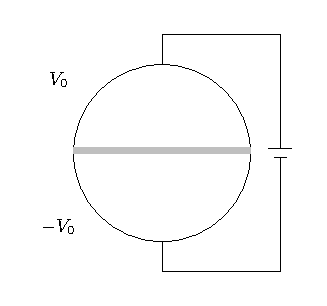
\includegraphics[scale=1.3]{Imagenes/Ejemplo_Esfera_03.eps}
\end{figure}

Se nos pide calcular el valor del potencial en puntos exteriores a la esfera, es decir, para puntos tales que $r > a$.
\par
El problema sigue manteniendo una simetría azimutal, conocemos ya la expresión que nos determina la solución, solo debemos de tomar en cuenta la condición que establece el problema.
\begin{align*}
\Phi (r, \theta) = \sum_{k=0}^{\infty} \left( A_{k} \, r^{k} + \dfrac{B_{k}}{r^{k+1}} \right) \, P_{k} (\cos \theta)
\end{align*}
Los coeficientes $A_{k}$ deben de anularse ya que se espera que el potencial se cancele en el infinito. Debiendo calcular entonces los coeficientes $B_{k}$.

\subsection{Una esfera dentro de otra esfera.}

Ahora consideremos el siguiente problema: Tenemos una esfera de radio $a$ formado por dos hemisferios a temperaturas $T_{1}$ y $-T_{1}$, éstos hemisferios están contenidos dentro de otra esfera de radio $b$, tal que $b > a$ y está a una temperatura $T_{2}$.
\begin{figure}[H]
    \centering
    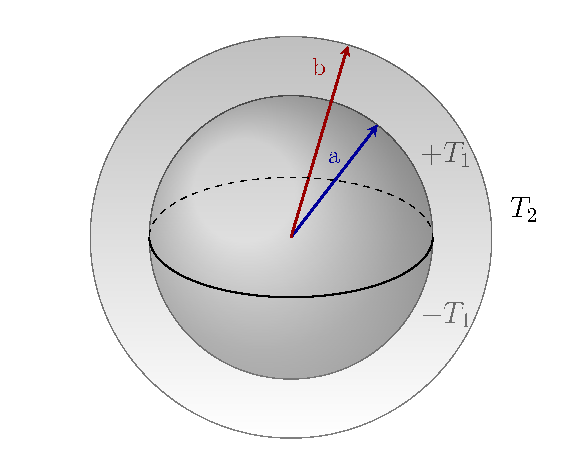
\includegraphics[scale=1]{Imagenes/Ejemplo_Esfera_02.eps}
\end{figure}

Se pide calcular la temperatura en:
\begin{enumerate}
\item Puntos interiores de la esfera de radio $a$: $r < a$.
\item Puntos entre la separación de las esferas: $a < r < b$.
\item Puntos exteriores de la esfera de radio $b$: $r > b$.
\end{enumerate}

Ya sabemos como abordar la solución en el caso para puntos interiores de la esfera de radio $a$ y para puntos exteriores de la esfera de radio $b$. Para los puntos intermedios debemos de considerar las condiciones de continuidad que marca el ejercicio, de tal manera que en esta parte si será necesario considerar ambos coeficientes de la expresión $\Phi(r,\theta)$ que se dedujo.
\end{document}